\documentclass[output=paper]{langsci/langscibook}
\ChapterDOI{10.5281/zenodo.3929245}


\markuptitle{Semantic and syntactic change of \textit{equis} in Mexican Spanish}{Semantic and syntactic change of equis in Mexican Spanish}
\renewcommand{\lsChapterFooterSize}{\small} %footers in editedvolumes
\renewcommand{\lsCollectionPaperFooterTitle}{Semantic and syntactic change of \noexpand\textit{equis} in Mexican Spanish}
\author{Olga Kellert\affiliation{Georg-August-Universität Göttingen}}

% \epigram{}

\abstract{In this paper, I investigate the synchrony and diachrony of the linguistic item \textit{equis} in Mexican Spanish. The origin of this item is the letter \textit{x} which stands for a variable. The item \textit{equis} has been recently used to refer to an utterance in the previous discourse which denotes a proposition and the speaker expresses his indifference with respect to this proposition, e.g. A: \textit{Es verdad.} ‘It’s true.’ B: \textit{Equis!} ‘I don’t care (whether it is true or not)’.

The diachronic change of \textit{equis} from a variable use \textit{x} into a discourse use is analyzed as a shift of indifference towards identities of atomic individuals into indifference towards truth values. This semantic shift is syntactically expressed as a shift from a nominal modifier into a sentence modifier. I will argue that only in the discourse use is the indifference lexically encoded.}

\begin{document}

\maketitle
% 1.
\section{Introduction}\label{sec:kellert:1}
In Mexican Spanish (Mex), the expression \textit{equis} stands for the character \textit{x} as in \REF{ex:kellert:1} which can be interpreted semantically as a variable ‘x’, if it is used as a nominal modifier as in \REF{ex:kellert:2}; (henceforth, the variable use of \textit{equis}):

% (1)
\ea\label{ex:kellert:1}
Equis o jota\\
\textit{`x} or \textit{j'}
\ex \label{ex:kellert:2}
Context: At some congress, scientists discuss the possibility of a planet on which life exists.\\
\gll Imaginemos un planeta \textbf{equis} donde viven otros seres humanos.\\
let-us-imagine a planet equis on-which live other beings humans\\
\glt `Let us imagine some planet x with human beings on it.'
\z

\textit{Equis} can also be used as a determiner (see also Diccionario del Español de México, DEM). In (\ref{ex:kellert:3}), \textit{equis} expresses that the speaker should be informed no matter what the reason for the addressee’s absence might be. In this context, \textit{equis} can be replaced by a free choice (FC) indefinite determiner \textit{cualquier} ‘any’ (see \citealt{AM2011} on \textit{cualquier} in European Spanish):

% (3)
\ea\label{ex:kellert:3}
\gll Si por \textbf{equis}/cualquier cosa no puedes venir mañana, házmelo saber.\\
if for equis/any thing not can come tomorrow let-me-it know\\
\glt ‘If for whatever reason you cannot come tomorrow, let me know.’ (Mex)
\z

Besides the determiner use of \textit{equis}, it can also have a predicative function with an Evaluative Interpretation of ‘unremarkable, unimportant’ in Mexican Spanish:

% (4)
\ea\label{ex:kellert:4}
\gll Así que es difícil identificar algo serio de algo \textbf{equis}.\\
so that is difficult indentifying something serious from something equis\\
\glt ‘It’s difficult to distinguish something serious from something unimportant.’
\z

It can also be used as a sentence or discourse adverb signaling speaker’s indifference with respect to the truth or falsehood of some proposition mentioned earlier in the discourse. The speaker B who utters \textit{equis} in (\ref{ex:kellert:5}) does not consider it important that the name under discussion is Nora:

% (5)
\ea\label{ex:kellert:5}
\begin{xlist}
\exi{A:}
\gll No es Dora, Es Nora.\\
not is Dora is Nora.\\
\glt ‘A: It’s not Dora, it’s Nora.’
\exi{B:}
\gll Equis!\\
equis\\
\glt ‘B: I don’t care!’
\end{xlist}
\z

As will be shown in the section on diachrony of \textit{equis}, these different uses did not arise simultaneously. The discourse adverb use appeared very late. The variable use appeared earlier than the discourse adverb use and it is restricted to written texts, whereas all other uses (determiner, predicative, discourse adverb use) are common in oral texts.

The main aim of this paper is to analyze the diachronic change of the linguistic item \textit{equis} and to investigate the possibility of analyzing all uses of \textit{equis}, or at least some of them, in a uniform way.
This study will shed some light on the relation between synchrony and diachrony and it will provide one possible answer to the question of how different synchronic meanings of one lexical item may develop diachronically.

This paper is organized as follows. I will first analyze the distribution of \textit{equis} and its functions on the basis of corpus data in synchrony (see \sectref{sec:kellert:2}). I will then suggest how to analyze different uses of \textit{equis} in a uniform way in \sectref{sec:kellert:3} and suggest a path about the diachronic development of different functions in \sectref{sec:kellert:4}. The suggested diachronic development will be then tested by diachronic data in \sectref{sec:kellert:5}. The summary and outlook will be presented in \sectref{sec:kellert:6}.

% 2.
\section{Syntactic and semantic functions of \textit{equis} in modern Mexican Spanish}\label{sec:kellert:2}
This section shortly describes different syntactic and semantic functions of \textit{equis} in Mexican Spanish according to the corpus data. Details will be presented in subsequent sections.

The synchronic data was taken from the \textit{Corpus del Español: Web\slash dialects} \citep{CDE}. 468 occurrences of \textit{equis} have been extracted from the synchronic corpus and classified according to syntactic and semantic/pragmatic features.

The relative frequency per million shows that the number of occurrences of \textit{equis} is higher in Mexican Spanish. (468 occ. per 260598272 occ. in total) than in other varieties of Latin American and European Spanish (for instance in Argentinian Spanish 218 occ. per 182704898 or in Europ. Sp. 418 occ. per 459312821).\footnote{It is impossible to use inferential statistics to compare the numbers in \tabref{tab:kellert:numbers} because these numbers represent numbers of populations and not means of different groups.}

\vfill
% (6)
\begin{table}
\caption{Number of occurrences of \textit{equis}\label{tab:kellert:numbers}}
\begin{tabular}{lS[table-format=3.0]S[table-format=9.0]S[table-format=1.1]}
\lsptoprule
Language & {Occurrences} & {Total} & {Per mil.}\\\midrule
Mex.Sp. & 468 & 260598272 & 1.8\\
Eu.Sp.  & 418 & 459312821 & 0.9\\
Arg.Sp. & 218 & 182704898 & 1.2\\
\lspbottomrule
\end{tabular}
\end{table}
\vfill
\pagebreak

The higher frequency of \textit{equis} in Mexican Spanish suggests that \textit{equis} is used in more numerous contexts in Mexican Spanish than in other varieties of Spanish.\footnote{Actually, a higher frequency in use of \textit{equis} in Mexican Spanish does not entail necessarily that \textit{equis} is used in more different contexts there. This is why I have tested speaker’s judgements as well.}  This suggestion is confirmed by the questionnaires with speaker's judgements according to which \textit{equis} is used in more contexts in Mexican Spanish than European Spanish, e.g. the discourse adverb use in (\ref{ex:kellert:7}) or the predicative use in (\ref{ex:kellert:8}):

% (7)
\ea\label{ex:kellert:7}
\begin{xlist}
\exi{A:}
\gll Oye, {¿}y si ya no te llama?\\
hey and if now not you call\\
\glt ‘A: Ey, what if (s)he doesn’t call you?'
\exi {B:}
\gll {¡}Ay, \textbf{equis}!\\
oh-my equis\\
\glt ‘B: Oh my, whatever!\slash forget about it!’\\
\end{xlist}
(8 Mex. speakers use \textit{equis} as discourse adverb, 5 Mex. speakers do not use it, but find the sentence grammatical, all 13 Europ. Spanish speakers find the sentence ungrammatical.)
\ex \label{ex:kellert:8}
\gll Es algo \textbf{equis}.\\
is something equis\\
\glt ‘It is something unimportant.’
(used by Mex. speakers, not used by European Spanish speakers)
\z

As one can see from the description of \textit{equis} in \tabref{tab:1:Equis MexSp. CDE}, which does not include the function of \textit{equis} as a proper noun (e.g. \textit{Signor Equis, rayos equis} ‘Mr. X, X-rays’)\footnote{I eliminated all occ. with \textit{equis} as a proper noun (209 occ.).}, \textit{equis} is mostly used as a nominal modifier (among 128 occ. of nominal modifier \textit{equis}, 105 occurrences as prenominal modifiers or determiners and 23 occurrences as postnominal modifiers). The second most frequent function is the discourse adverb function (49 occ.), followed by the predicative use of \textit{equis} with copular(like) verbs (9 occ.).

In most cases, \textit{equis} appears in sentences with verbs in present tense. The most frequent interpretation of \textit{equis} is the expression of the speaker’s ignorance (Ignor.) and/or Indifference (Indif.) ‘I don’t care about x’ (see \tabref{tab:1:Equis MexSp. CDE}).

% Tabelle 1
\begin{table}\small
\caption{\textit{Equis} in Mexican Spanish in CDE web/dialects}
\label{tab:1:Equis MexSp. CDE}
 \begin{tabularx}{\textwidth}{CCCCC}
  \lsptoprule
   \multicolumn{5}{c}{{Syntactic Function}}\\
  \midrule
  \multicolumn{2}{p{5cm}}{\centering Nominal modifier/Determiner\linebreak(128 in total)} &  Predicate (e.g. \textit{Es equis})  &    Discourse adverb & Total\\\cmidrule(lr){1-2}
  \textit{Equis} N  &   N \textit{Equis} &  & \\
  \midrule
  {105}  &   {23} &   {9} &    {49} & 181\\
  \midrule\tablevspace\tablevspace
 \end{tabularx}
 \begin{tabularx}{\textwidth}{CCCCCC}
   \multicolumn{6}{c}{{Tense and Mood}}\\
  \midrule
 Present tense & Past tense & Subj.\slash Condit. & Modal verb & Imperative & Total\\
  \midrule
  {64} & {37}  &   {14} &   {16} &    {1} & 132\\
  \midrule\tablevspace\tablevspace
 \end{tabularx}
 \begin{tabularx}{\textwidth}{CCCCC}
   \multicolumn{5}{c}{{Interpretation}}\\
  \midrule
 Ignor.\slash Indif. & Eval. ‘unimp.’ & ``Various'' & ``Certain'' & Total\\
  \midrule
  {111} & {24}  &   {9} &   {38} & 181\\
  \lspbottomrule
 \end{tabularx}
\end{table}

The details of every syntactic and semantic function are discussed in the following subsections.

% 2.1
\subsection{\textit{Equis} as prenominal modifier or determiner}\label{sec:kellert:2.1}
The prenominal modifier or determiner \textit{equis} has the function of an existential quantifier ‘some’ when used with respect to the number or quantity of the noun it modifies (e.g. \textit{equis pesos} ‘some cents’, \textit{equis número de coches} ‘some number of cars’, \textit{equis cantidad} ‘some quantity’, \textit{equis años} ‘some years’. There are no occurrences with the prenominal \textit{equis} preceded by an article (e.g. \textit{un, a} ‘a’). This observation suggests that \textit{equis} acts as a determiner in the prenominal position.

As will be shown in the following data, tense and modality matter for the interpretation of \textit{equis}. If \textit{equis} appears in free choice (FC) contexts (e.g. generic sentences, conditional antecedent, comparatives, etc. see \citealt{Aloni2010} for FC contexts), it has FC interpretation (i.e. every alternative is a possible option):\footnote{In order to be sure that \textit{equis} has FC interpretation in FC contexts, native speakers of Mexican Spanish were asked if they could also use \textit{cualquier} instead of \textit{equis} in these contexts (for FC interpretation of cualquier, see \citealt{AM2011}, among others).}

% (9)
\ea\label{ex:kellert:9}
\gll Si para tu abuelo es importante que lo acompañes \textbf{a} \textbf{equis} \textbf{lado}, acompáñalo a \textbf{equis} lado.\\
if for your grandfather is important that him accompany to equis place accompany-him to equis place\\
\glt ‘If it is important for your grandfather to go with him anywhere, go with him anywhere.’
\ex 
\gll de modas o creación de una necesidad innecesaria - en el caso de verse \textbf{como} \textbf{equis} \textbf{tv-star}, porque se pierde la verdadera identidad del o personal.\\
of trends or creation of a necessity innecesary {} in the case of seeing-oneself as equis tv-star because it	loses the true identity of.fes unnthe self personal\\
\glt ‘Regarding trends or creating unnecesary needs – in the case of seeing oneself as \textit{any} TV-star, because you loose the true identity of your personal self.’
\z

In episodic sentences, the determiner \textit{equis} refers to some specific individual (e.g. some artist) with an ignorance or indifference inference, i.e. the speaker signals that he/she does not remember or know the name of the artist or does not find it important to mention it:

% (11)
\ea\label{ex:kellert:11}
\gll  Pero la última vez que estuve allá, fue en un concierto de \textbf{equis} \textbf{artista} donde estábamos yo y cuatro personas más. Era patético.\\
but the last time that was there was in a concert of equis artist where were me and four people more was pathetic
\\
\glt ‘But the last time I was there, it was at a concert of some artist where it was me and four people more. It was pathetic.’
\z

In sentences with negation as in (\ref{ex:kellert:12}), \textit{equis} either refers to some reason with ignorance inference as in (\ref{ex:kellert:11}) or it has a universal interpretation as in (\ref{ex:kellert:13}) where the addressee is asked to inform the speaker for every reason there is that prevents the addressee from coming:

% (12)
\ea \label{ex:kellert:12}
\gll  pero en definitiva es una opción para las familias que por \textbf{equis} \textbf{motivos} no tienen oportunidad de salir de vacaciones.\\
but in end is an option for the families that for equis reason not have oportunity of going-out of holidays\\
\glt ‘But, in the end, it is an option for families that, for some reason, don’t have the opportunity to go on holiday.’
\ex \label{ex:kellert:13}
\gll  Si por \textbf{equis} \textbf{razón} no vas a venir, avisame.\\
if for equis reason not go to come inform-me\\
\glt ‘If for whatever reason you cannot come, inform me.’
\z

The determiner \textit{equis} is much more flexible with interpretations than usual FC indefinites such as Sp. \textit{cualquier} ‘any’. It can have the meaning of ‘much/a lot’ which seems to be context dependent, especially in contexts that trigger the interpretation of long duration, e.g. \textit{equis tiempo} ‘long time’ (see \citealt{Rivero2011} for a similar observation on \textit{cualquier cuantidad} ‘any quantity’ or ‘a lot of quantity’):

% (14)
\ea\label{ex:kellert:14}
\gll Sí, soy divorciado. -- Sí, hace \textbf{equis} tiempo.\\
yes am divorced {} yes ago equis time\\
\glt ‘Yes, I’m divorced. -- Yes, a long time ago.’
\z

It can also mean ‘several’ or ‘many’ when it appears with plural NPs:

% (15)
\ea\label{ex:kellert:15}
\gll  Antes uno para una promoción esperaba \textbf{equis} \textbf{años}.\\
before one for a promotion waited equis years\\
\glt ‘In the past, you had to wait many years to be promoted.’
\ex 
\gll  o como si fuera una estación de subte que tiene \textbf{equis} \textbf{estaciones} y cada estación se ocupa de sus usuarios\\
or like if was a station of subway that has equis stations and each station it attends of its users\\
\glt ‘Or as if it were a subway station that has several stations and each one attends to its users.’
\z

The meaning ‘much/many/several’ also has an ignorance or indifference interpretation, i.e. the speaker does not know the identity or the exact number of the variable x or the speaker does not find it important to mention the identity or the number of the variable x.
To summarize this section about prenominal or determiner \textit{equis}, it acts as an indefinite ‘some’ and depending on the modal or episodic context, it can either have FC interpretation or be interpreted as an indefinite with an ignorance/indifference interpretation. \textit{Equis} can have the meaning of ‘several’ or ‘many’, if it modifies plural nouns.

% 2.2
\subsection{Adjectival or predicative use of \textit{equis}}\label{sec:kellert:2.2}
The corpus data contain examples with \textit{equis} after copular(-like) verbs (\textit{ser\slash estar} ‘be-stative’, \textit{volver} ‘become’) with the meaning ‘neither good nor bad\slash unremark\-able’ in (\ref{ex:kellert:17}) or ‘unimportant’ in (\ref{ex:kellert:18}):

% (17)
\ea\label{ex:kellert:17}
\begin{xlist}
\exi{A:}
\gll {¡}Hola! {¿}Qué tal estuvo la película que fuiste a ver ayer?\\
hello how so was the film that went to see yesterday\\
\glt `Hey! How was the movie yesterday?'
\exi{B:}
\gll  Estuvo \textbf{equis}, me esperaba algo mejor.\\
was equis I expected something better\\
\glt `The movie was unremarkable. I expected something better.’
\end{xlist}
\ex \label{ex:kellert:18}
\gll  Ese chavo me es \textbf{equis}.\\
this guy me is equis\\
\glt ‘This guy is not important to me./I don’t care about this guy.’
\z

The predicative \textit{equis} can be modified by degree adverbs \textit{muy, tan, bien, bastante, completamente} ‘very/completely’ usually denoting high degrees:

% (19)
\ea\label{ex:kellert:19}
\gll Cuando conocí a René me pareció \textbf{muy} \textbf{equis}, o sea, como insignificante, un nerd.\\
when met with René to-me seemed very equis that is like insignificant a nerd\\
\glt ‘When I got to know René, he appeared very unremarkable/normal to me, or insignificant, a nerd.’
\ex 
\gll La comida no es mala pero es \textbf{muy} \textbf{equis}.\\
the food not is bad but is very equis\\
\glt ‘The food is not bad but very ordinary.’
\z

When \textit{equis} is used under negation, the negation expresses that it is not the case that some individual holds an unremarkable or a bad property, but rather a good or a distinguished property.

% (21)
\ea\label{ex:kellert:21}
\gll \textbf{No} \textbf{está} \textbf{equis}. Es una galería linda.\\
not is equis is a gallery beautiful\\
\glt ‘It [=the gallery] is not bad/ordinary. It is a beautiful gallery.’
\z

% 2.3
\subsection{Postnominal \textit{equis}}\label{sec:kellert:2.3}
The postnominal \textit{equis} is less frequent than the prenominal one (four times less). All occurrences found in the corpus with postnominal \textit{equis} are restricted to indefinite or bare nouns (e.g.  \textit{motivos equis} ‘reasons x’, \textit{una mujer equis} ‘a woman x’).\largerpage

When postnominal \textit{equis} appears after a copular(-like) verb, it is interpreted as a gradable adjective with the meaning ‘ordinary, unimportant’ and can be modified by degree adverbs like \textit{muy, bastante}, ‘very’ (see also the adjectival use of \textit{equis} in \sectref{sec:kellert:2.2}):

% (22)
\ea\label{ex:kellert:22}
\gll  es una mujer (muy) \textbf{equis}, sorry pero sí lo es.\\
is a woman (very) equis sorry but yes it is\\
\glt ‘She is a (very) ordinary woman. I’m sorry but she is.’
\ex 
\gll  Una fiesta (bastante) \textbf{equis}.\\
a party (very) equis\\
\glt ‘a (very) unremarkable party’
\z

When postnominal \textit{equis} occurs in modal contexts (e.g. with modal verbs), it usually has the interpretation of an FCI ‘any’ (see also prenominal \textit{equis} in \sectref{sec:kellert:2.1}):

% (24)
\ea\label{ex:kellert:24}
\gll  Así, en un momento dado, un país \textbf{equis} puede estar generando ahorro, pero este puede filtrarse hacia el exterior;\\
so in a momento given a country equis can be generating savings but this can leak towards the exterior\\
\glt ‘In that way, at one point, any country may save money, but this money can leak out.’
\z

If postnominal \textit{equis} appears in episodic contexts that refer to past events, postnominal \textit{equis} can have the interpretation of a variable x as in (\ref{ex:kellert:25}) and (\ref{ex:kellert:26}). In (\ref{ex:kellert:25}), the speaker does not specify the exact reasons for why she stopped drinking and the hearer infers that these reasons are unimportant to be mentioned for the main argument of the discussion, namely that she lost weight. Note that in this context, degree modification of \textit{equis} as with adjectival use of \textit{equis} (see \sectref{sec:kellert:2.2}) would not make much sense, because the argument of the discussion is not about the speaker's evaluation of the reasons but about losing weight:

% (25)
\ea\label{ex:kellert:25}
\gll  Estuve tomando por espacio de dos meses, deje de tomar por motivos \textbf{equis} y de un tiempo a esta parte fui a la balanza y hoy estoy pesando 120 kilos.\\
was drinking for space of two months quit of drinking for reasons equis and from some time to this side was to a scale and today am weighing 120 kilos\\
\glt ‘I was drinking for two months, I quit for reasons x and, for some time, I weighed myself on the scales and now I weigh 120 kilos.’
\z

In the following context, the hearer infers from the variable use of \textit{equis} that the speaker is ignorant or indifferent about the deasease with which every child was born. As in (\ref{ex:kellert:25}), degree modification does not make sense here either:

% (26)
\ea\label{ex:kellert:26}
\gll  Uno se entera de cada caso de niños que nacieron con una enfermad \textbf{equis}, a destiempo, de bajo peso, que se tienen que quedar en incubadora.\\
one it learns of each case of children that were-born with a disease equis a wrong-time of little weigh that them have to stay in incubator\\
\glt ‘One learns about each case of children who are born \textit{with a disease x}, at the wrong time, with little weigh, and they have to remain in the incubator.’
\z

The variable use is always replacable by the character x or some other character (e.g. \textit{una enfermedad x o z} ‘a disease x or z’).

To sum up, \textit{equis N} and \textit{un,a N equis} can have a similar meaning of ‘some’ or ‘any’ despite their different syntactic status. This is due to the possibility of interpreting \textit{equis} in \textit{un,a N equis} as ‘some’ in episodic contexts or as ‘any’ in modal contexts. Under copular(-like) verbs postnominal \textit{equis} is always interpreted as a degree predicate with the meaning ‘unremarkable, unimportant’ which can be degree modified. In this case, the postnominal \textit{equis} cannot be replaced by the character x.

% (27)
\ea[*]{\label{ex:kellert:27}
\gll es una fiesta muy x (o z)\\
     is a party very x (or z)\\}
\z

To conclude, postnominal \textit{equis} can have an adjectival function with an evaluative interpretation of ‘unremarkable, unimportant’ in predicative position or it can be interpreted as a variable x and additionally express speaker’s indifference or ignorance about the value of x.

% 2.4
\subsection{Discourse adverb use}\label{sec:kellert:2.4}
The discourse adverb \textit{equis} is different from all other functions shown so far as the discourse adverb \textit{equis} must not appear inside a clause and be adjacent to some category it modifies:

% (28)
\ea\label{ex:kellert:28}
\begin{xlist}
\exi{A:} {\itshape No es Dora, es Nora, teto}\\
\exi{B:} {\itshape Equis}\\
\exi{A:} {\itshape Pues}\\
\glt ‘A: It’s not Dora, it is Nora, looser. - B: I don’t care! - A: Well…’
\end{xlist}
\z

% (29)
\ea\label{ex:kellert:29}
\gll Sí son homosexuales, \textbf{equis}. O heterosexuales, \textbf{equis}, el punto es respetarse a sí mismo.\\
if are homosexuals equis or heterosexuals equis the key is respecting to one self\\
\glt ‘If they are homosexual, I don’t care, or heterosexual, I don’t care, the most important is to respect oneself.’
\z

As a discourse adverb, it can have several functions, one of which is to express that the speaker does not care about which alternative proposition is true. In (\ref{ex:kellert:28}) the speaker signals that he does not care whether the name of some girl is Dora or Nora. In (\ref{ex:kellert:29}), the speaker expresses his indifference as to which answer is true, i.e. the speaker is indifferent about whether they are homosexuals or not, it does not matter as long as everyone respects each other. To sum up, the discourse adverb \textit{equis} expresses speaker’s indifference with respect to the truth of alternative propositions.

There is no discourse adverb \textit{equis} with degree modification in the corpus data in contrast to the predicative/adjectival use of \textit{equis} in (Sections~\ref{sec:kellert:2.2} and~\ref{sec:kellert:2.3}):

% (30)
\ea\label{ex:kellert:30}
\begin{xlist}
\exi{A:} Some utterance \textit{x} \\
\exi{B:} \textit{Muty equis.} (0 occ. in CDE)\\
\glt ‘I don’t care (a lot) about utterance x.’
\end{xlist}
\z

Moreover, the discourse adverb \textit{equis} cannot be negated in contrast to the predicative use of \textit{equis} (see e.g. \ref{ex:kellert:31}):
% (31)
\ea\label{ex:kellert:31}
\begin{xlist}
\exi{A:} You don't seem to care about \textit{x}. \\
\exi{B:} \textit{No equis.} (0 occ. in CDE)\\
         \glt 'It's not true that I don't care about x.= I do care about x'
\end{xlist}
\z

The discourse adverb \textit{equis} can also appear as a reaction to a question being addressed by the interlocutors in a given discourse where the speaker signals that he is not interested in the right answer to the question being discussed, i.e. he is indifferent towards any answer to the current question under discussion (QUD; see \citealt{Roberts1996}):

% (32)
\ea\label{ex:kellert:32}
\gll Porque siento que alguien más lo ha dicho mejor que yo, pero \textbf{equis}, si me pides mi opinión, yo diría que…\\
because feel that someone more it has said better than me but equis	if me ask my opinión I would-say that\\
\glt ‘Because I think somebody said it better than me, but I don’t care. If you ask my opinion, I would say that…’
\ex 
\gll  {¿}Cómo	estás? Igual, \textbf{equis}. Bien. {¿}Cómo están tus jefes?\\
how are same equis good how are your bosses\\
\glt ‘How are you? The same, but it’s not important. Good. How are your parents?’
\z

Besides expressing the indifference towards some (hidden) alternatives, it can have a discourse function signaling a topic change in the discussion. Usually, this function is expressed by \textit{pero equis, ay equis, bueno, equis} ‘But, well, anyway/whatever’:

% (34)
\ea\label{ex:kellert:34}
\gll ¡Hola! Hoy es el primer día de clases así que estoy emocionada traumada pero \textbf{equis}, todo va bien por el momento (luego nos aplastarán como cucarachas).\\
hello today is the first day of classes so that am excited shocked but equis all goes well for the moment later us smash like cockroaches\\
\glt ‘Hello! This is the first day of classes so I am very exited but anyway, everything is going well for the time being (then they will smash us like cockroaches).’
\ex 
\gll está bien fea tu ciudad alcranienta... bueno \textbf{equis} disculpa que sea grosero pero pues asi somos los chilangos de categoria\\
is very ugly your city alcranienta well equis sorry that be.\textsc{subj} rude but well so are the chilangos of high-rank\\
\glt ‘It is so ugly your “alcranienta” city. Anyway, sorry for being so rude but we Mexicans are like that.’
\z

To sum up, \textit{equis} as discourse adverb expresses speaker’s indifference towards the right answer to the current QUD or towards whatever has been said in the previous discourse.

% 2.5
\subsection{Summary of the data and further outlook}\label{sec:kellert:2.5}\largerpage[-1]
According to the description of the synchronic data, \textit{equis} as a determiner has the meaning ‘some, certain, various’ and as a postnominal modifier \textit{equis} has a variable use x which is interpreted as ‘some’ with ignorance/indifference inference in episodic contexts (e.g. \textit{motivos x} ‘some reasons’ and I don’t know/care which ones). In modal contexts, it is interpreted as a free choice ‘any’. In predicative position after copular(-like) verbs, \textit{equis} has an adjectival use with the possibility of degree modification (e.g. \textit{muy equis} ‘very unremarkable\slash bad\slash unimportant’). As discourse adverb, \textit{equis} expresses the speaker’s indifference with respect to a proposition which corresponds to an answer to some QUD (see \tabref{tab:4:Summary contexts}).

% Tabelle 2
\begin{table}\footnotesize
\caption{Summary of contexts, syntactic categories, semantic/pragmatic functions\label{tab:4:Summary contexts}}
 \begin{tabularx}{\textwidth}{p{2cm} p{2.75cm} C C C C}
  \lsptoprule
     &  &  \multicolumn{4}{c}{Syntactic category}\\\cmidrule(lr){3-6}
  \raggedright {Syntactic contexts}  & {Interpretations\slash Functions} & {Deter\-miner} & {Post-nominal} & {Sentential adverb} & {Predicate}\\
  \tablevspace
     & \raggedright Variable use (x or z) + ignorance or indifference & $-$ & $+$ & $-$ & $-$\\
  \tablevspace
   \raggedright Episodic contexts $\lbrace$perfective past$\rbrace$  & \raggedright Existential quantifier ‘some’ +  ignorance or indifference with plural NP ‘some, many, various’ & $+$ & $-$ &  & $-$\\
  \tablevspace
   \raggedright Modal contexts $\lbrace$if-clauses, generic sentences$\rbrace$ & free choice ‘any’ & $+$ & $+$ & $-$ & $-$\\
  \tablevspace
   \raggedright Predicative contexts $\lbrace$copula clauses$\rbrace$ & \raggedright Degree predicate ‘unimportant, unremarkable’ & $-$ & $+$ & $-$ & $+$\\
  \tablevspace
   \raggedright Not embedded in a sentence  & \raggedright ‘I don’t care’ & $-$ & $-$ & $+$ & $-$\\
  \lspbottomrule
 \end{tabularx}
\end{table}

As one can easily see, the indifference inference appears almost everywhere. It is somewhat parasitic on the indefinite and variable use of \textit{equis}. It is lexicalized as a degree predicate ‘unimportant’ under copular(-like) verbs and it is expressed by the meaning ‘I don’t care’ of the discourse adverb. The main working hypothesis is thus that the indifference inference is the core property of (almost) every use of synchronic \textit{equis}. It makes sense to suggest a unified analysis of \textit{equis} based on the indifference inference and to explain the variation between different uses synchronically (\sectref{sec:kellert:3}) and diachronically (\sectref{sec:kellert:4}).

% 3.
\section{Synchronic analysis of \textit{equis}}\label{sec:kellert:3}
In \sectref{sec:kellert:2}, the data have shown that the notion of indifference is the common interpretation associated with many uses of \textit{equis}. I will first introduce into the notion of von Fintel’s indifference \cite{Fintel2000} in \sectref{sec:kellert:3.1}. I will then apply this notion to the variable use of \textit{equis} in \sectref{sec:kellert:3.2}, the discourse adverb \textit{equis} in \sectref{sec:kellert:3.3} and the postnominal \textit{equis} in \sectref{sec:kellert:3.4}.

% 3.1
\subsection{Von Fintel’s indifference}\label{sec:kellert:3.1}
One prominent analysis of indifference was suggested by \citet{Fintel2000} for the English indefinite \textit{wh-ever} (see also \citealt{Condoravdi2005}). The indifference inference in the following example is expressed as a presupposition according to which the agent Ed could have blurted out anything else:

% (36)
\ea\label{ex:kellert:36} 
    \textit{In response, Ed blurted out whatever came to his mind first.}\\
	Assertion: In response, Ed blurted out the first thing that came to his mind.\\
	Presupposition: Ed could well have blurted out anything else that came to his mind first.
\z

Under \citegen{Fintel2000} analysis in (\ref{ex:kellert:37}), the presuppositional content of \textit{whatever} makes reference to a contextually determined modal base F, a mapping from worlds to sets of worlds (see \ref{ex:kellert:37}). F(w) is the set of worlds in which the speaker' s beliefs about w hold. Sim expresses similarity between worlds and maps a world w and a proposition p to a set of worlds maximally similar to w in which p is true. The presupposition triggered by \textit{whatever came to his mind first} conveys that if the thing that came to his mind first had been different in all the counterfactual worlds, the truth of the proposition “Ed blurted out the thing that came to his mind first” would also hold in the counterfactual world (see \citealt{Condoravdi2005}).

% (37)
\ea\label{ex:kellert:37} indifference analysis \citep{Fintel2000}\\
whatever(w)(F)(P)(Q)
\begin{xlist}
\ex presupposes:\\
{($\forall$w’ $\in$ Sim (w, F(w)) $\cap$ ($\lambda$ w”. ίx. P (x,w”) ≠ ίx. P (x,w))
	Q(w’)(ίx. P (x,w’)) = Q(w)(ίx. P (x,w))}
\ex	asserts:\\
{Q(w)(ίx. P (x,w))}
\end{xlist}
\z

On von Fintel’s analysis, whatever-statements presuppose that the speaker cannot identify the referent of the free relative and assert that the referent -- whatever it is -- has the matrix property in all of the speaker's alternatives (see \citealt{Condoravdi2005}). According to \cite{Fintel2000}, ignorance and indifference inferences are the result of different modal bases: in case every alternative is a possible alternative according to the speaker’s knowledge, the ignorance inference is triggered. In case every alternative is a possible alternative according to the speaker's preferences, the indifference inference is triggered.

Whether a \textit{wh-ever} free relative has an external indifference or agent indifference interpretation depends on contextual factors, and is only an “epiphenomenal inference” that is drawn from the presupposition of variation, i.e. from the presupposition that every alternative is a possible option (\citealt[108]{Tredinnick2005}). On Tredinnick’s analysis whenever there is no overt expression of an agent, the indifference is speaker related (e.g. I blurted out whatever came to my mind first.). This is indeed what has been observed in the literature on Spanish FCI \textit{cualquiera}. If \textit{cualquiera} is embedded under volitional verbs that express some volitional agent, it expresses agent's indifference with respect to the choice of some alternative (see \citealt{CR2008}, \citealt{AM2011}). In the following example, the agent’s indifference refers to the choice of the book:

% (38)
\ea\label{ex:kellert:38}
\gll Juan necesitaba un pisapapeles, de modo que cogió un libro cualquiera.\\
Juan needed a paperweight of way that he-took a book cualquiera\\
\glt ‘Juan needed a paperweight, so he took a random book.’
\z

I suggest to derive the indifference of the variable use of \textit{equis} from von Fintel's counterfactual inference (see variable use of \textit{equis} in 3.2).

% 3.2
\subsection{Variable use of \textit{equis}}\label{sec:kellert:3.2}
I assume the following syntax of the variable use of \textit{equis} represented as x in order to distinguish it from other uses such as the discourse adverb use. The postnominal x is represented as a reduced relative clause similar to postnominal adjectives in Romance and other languages (see \citealt{Cinque:2010} and others) in \figref{fig:kellert:tree1n}.\pagebreak

% BAUM 1
%\begin{center}
%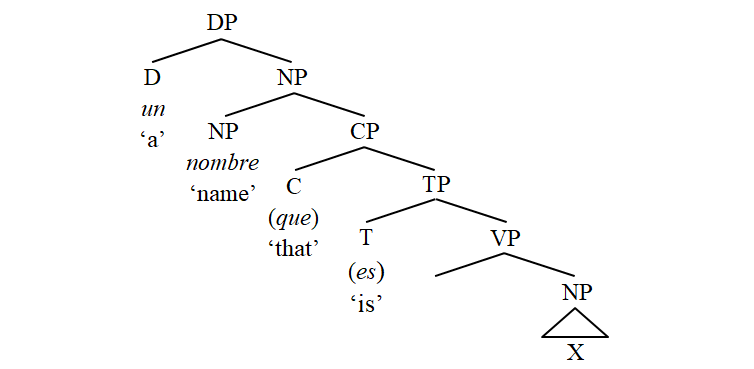
\includegraphics[scale=0.5]{figures/tree1n.png}
% \captionof{figure}{Syntax of the variable \textit{equis}}
%\end{center}

\begin{figure}
	\begin{forest}
		[DP
			[D\\\textit{un}\\`a'] [NP
				[NP\\\textit{nombre}\\`name'] [CP
					[C\\(\textit{que})\\`that'] [TP
						[T\\(\textit{es})\\`is'] [VP
							[~] [NP [$X$,roof]]
						]
					]
				]
			]
		]
	\end{forest}
	\caption{Syntax of the variable \textit{equis}\label{fig:kellert:tree1n}}

\end{figure}

The DP as represented in Figure \ref{fig:kellert:tree1n} denotes some name. Additionally, the variable x adds the information that x is a specific name, say \textit{Dora} or \textit{Nora} (see \ref{ex:kellert:39b}). I represent the requirement that x is a specific name as a set of domain alternatives which is exhaustified, i.e. only one alternative can hold (see \ref{ex:kellert:39c}):

% (39)
\ea\label{ex:kellert:39} The denotation of \textit{un nombre x}:
\begin{xlist}
\ex\label{ex:kellert:39a}
{\textlbrackdbl \textit{un nombre x}\textrbrackdbl = $\lambda$P $\exists$x $\in$ D [name(x) $\wedge$ P(x)]}\\
in words: ‘some name’
\ex\label{ex:kellert:39b}
{Domain Alternatives(DA) = $\lbrace$$\lambda$P $\exists$x $\in$ D’ [name(x) $\wedge$ P(x)] | D’ $\subseteq$ D$\rbrace$}\\
in words : $\lbrace$Dora, Nora$\rbrace$ where Dora, Nora are alternatives of ‘some name’
\ex\label{ex:kellert:39c}
Exhaustification of domain alternatives=x is either Dora or Nora.
\end{xlist}
\z

If the denotation in (\ref{ex:kellert:39}) is applied to the rest of the whole sentence in (\ref{ex:kellert:40}a), the result is an assertion in (\ref{ex:kellert:40}b). (\ref{ex:kellert:40}c) represents a set of alternatives applied to propositions. The exhaustification in (\ref{ex:kellert:40}d) expresses that only one alternative proposition is true in the world of evaluation:

% (40)
\ea\label{ex:kellert:40}
\begin{xlist}
\ex Tiene un nombre \textit{equis}  ‘She has a name x’\\
\ex Assertion: $\exists$x [x is a name and she/he has some name(x)]\\
\ex Alt = $\lbrace$her name is Dora, her name is Nora$\rbrace$\\
\ex Exhaust(Alt) = $\lbrace${[}$\lambda$w: Her name is Nora and not Dora in w{]} ; {[}$\lambda$w: Her name is Dora and not Nora in w{]}$\rbrace$\\
\end{xlist}
\z

I assume that (\ref{ex:kellert:40}a) expresses speaker's indifference with respect to the value of the variable x which follows from the counterfactual inference in (\ref{ex:kellert:41}), namely that if her name had been different in all the counterfactual worlds, the truth of the proposition that she has some name would still hold in the counterfactual worlds:

% (41)
\ea\label{ex:kellert:41}
Counterfactual inference associated with the variable x:\par
($\forall$w’ $\in$ Sim (w, F(w)) $\cap$ ($\lambda$w”. x: name (x,w”) $≠$ x: name (x,w)) \par
$\exists$x.name (x,w’) \& be (her, x, w’) = $\exists$x.name (x,w) \& be (her, x, w)\\
\glt ‘No matter what her actual name is, all names are equal.’
\z

The question is where the counterfactual inference in (\ref{ex:kellert:41}) comes from. Is it lexically encoded in the variable use or does it follow from some pragmatic principle? I assume that it is a pragmatic inference that goes informally as follows. The hearer concludes from (\ref{ex:kellert:40}a). that it does not matter to the speaker which of the alternatives triggered by x holds in the actual world because if the speaker knew the name of the person he would have said so due to Gricean conversational maxims (roughly: be informative, say true things, be relevant) (see \citealt{Aloni2005} for formal analysis of Gricean implicatures). The indifference inference derived from the variable use of \textit{equis} has a similar pragmatic status as disjunctions or plain indefinites (see \citealt{Aloni2005} for the indifference inference associated with these items).

% (42)
\ea\label{ex:kellert:42} \textit{Do you want coffee or tea?}
\par
Pragmatic inference: The speaker does not have any preference as to whether I, hearer, should take coffee or tea.
\ex  \textit{Paul married some girl from Nebraska.}
\par
Pragmatic inference: Hearer assumes that the speaker is ignorant about the 	identity of the girl or he does not consider it important to mention her name.
\z

I assume that the indifference inference associated with the variable use x is not lexically encoded in the lexical entry of x itself but is derived as a pragmatic inference according to which every value for the variable x is a possible candidate for the truth of the proposition.

% 3.3
\subsection{Degree predicate analysis of \textit{equis}}\label{sec:kellert:3.3}
In the following example the postnominal \textit{equis} is neither interpreted as a variable nor as a discourse adverb \textit{equis} but as a predicative adjective with the meaning ‘unimportant’ as it is contrasted to the meaning ‘serious’.

% (44)
\ea\label{ex:kellert:44}
\gll Así que es difícil identificar algo serio de algo \textbf{equis}.\\
so that is difficult indentifying something serious from something	equis\\
\glt ‘It’s difficult to distinguish something serious from something unimportant.’
\z

The predicative \textit{equis} can be degree modified:

% (45)
\ea\label{ex:kellert:45}
\gll Estuvo bien \textbf{equis}.\\
was very equis\\
\glt `It was very ordinary/unimportant.’
\z

The degree analysis of \textit{equis} as ‘unimportant’ is represented as follows. The predicate \textit{equis} takes a degree argument d, an individual x and an attitude holder s (usually the speaker) and states that x is unimportant or ordinary to degree d to s (see Figure \ref{fig:kellert:tree2}):

% (46)
\ea\label{ex:kellert:46} {[}Adv/Adj \textit{equis}{]} = $\lambda$d$\lambda$x. \textit{ordinary/unimportant to s to degree} (d)(x)
\z

The degree predicate can be modified by degree adverbials such as \textit{muy/tan/bien} that denote high degrees:

% (47)
\ea\label{ex:kellert:47} {[}DeP Deg° \textit{muy/tan/bien} ‘very’ {[}Adv/Adj equis{]]}  = $\lambda$x. very \textit{ordinary/unimportant}’ (x)
\z

I assume that \textit{algo equis} in (\ref{ex:kellert:44}) is represented as a small clause (PrP) that denotes a proposition that something is ordinary/unimportant to some degree d to some attitude holder s.

% (48)
\ea\label{ex:kellert:48} {[}PrP algo equis{]}  =  $\lambda$d $\exists$x. ordinary/unimportant to s to degree (d) (x)
\z

% BAUM 2
%\begin{center}
%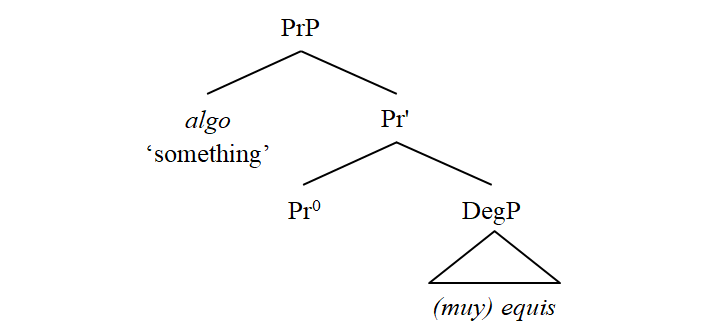
\includegraphics[scale=0.5]{figures/tree2.png}
% \captionof{figure}{Syntax of the degree predicate \textit{equis}}
%\end{center}
\begin{figure}
	\caption{Syntax of the degree predicate \textit{equis}\label{fig:kellert:tree2}}
	\begin{forest}
		[PrP
			[\textit{algo}\\`something'] [Pr'
				[Pr\textsuperscript{0}] [DegP
					[\textit{(muy) equis},roof]
				]
			]
		]
	\end{forest}
\end{figure}

The syntax of the adjectival use of \textit{equis} and the variable x (see Figure \ref{fig:kellert:tree1n}) are almost identical. They both represent predicative elements. However, they are semantically different. In the degree predicate use, the term \textit{equis} is interpreted as a degree predicate. In the variable use, \textit{equis} is a predicate that is identical with a specific element of the set denoted by the noun.


% 3.4
\subsection{Discourse use of \textit{equis}}\label{sec:kellert:3.4}
In order to represent the syntactic structure of the discourse adverb \textit{equis} in (\ref{ex:kellert:49}), I assume that \textit{equis} adjoins to the sentence that serves as an answer to the QUD in (\ref{ex:kellert:50}) (i.e. \textit{what is her name?}):

% (49)
\ea\label{ex:kellert:49} A: \textit{No es Dora, Es Nora.} `It’s not Dora, it’s Nora.' B: \textit{Equis}! ‘I don’t’ care!’
\ex\label{ex:kellert:50}  \textit{Equis} {[}It is Nora\textsubscript{Focus}{]} ‘I don’t care whether it’s Nora or not.’
\z

\textit{Equis} can be used as a sentential adverb that selects a sentence with a focus feature. The focus feature generates alternatives (i.e. her name is Nora or some other name):

% (51)
\ea\label{ex:kellert:51} Alt(S) = $\lbrace${[}$\lambda$w: Her name is Nora in w{]}; {[}$\lambda$w: Her name is Dora in w{]}$\rbrace$
\z

The function of \textit{equis} is to express indifference with respect to these alternatives, i.e. the speaker is indifferent as to which alternative is the right answer to the current QUD (i.e. \textit{what is her name}).

The discourse adverb \textit{equis} has the following denotation. It takes a context variable (c), a world-time variable (i), a set of alternative propositions that represent some QUD, a speaker (s) and an addressee (a). The discourse adverb expresses speaker’s indifference at some context c and world-time (i) to the addressee (a) about every proposition of QUD:

% (52)
\ea\label{ex:kellert:52} $\parallel$Discourse Adverb Equis$\parallel$ (c)(i) (QUD\textsubscript{{<}{<}st>t>}) (s)(a) =\par at time-world index i and in a context c, the speaker s expresses his indifference to the addressee a about $\forall$q\textsubscript{<st>} $\in$ QUD\textsubscript{{<}{<}st>t>}
\z

If the denotation in (\ref{ex:kellert:52}) is applied to the sentence in (\ref{ex:kellert:49}), the result is the following denotation which expresses speaker’s indifference wrt alternative proposition represented in (\ref{ex:kellert:51}):

% (53)
\ea\label{ex:kellert:53} $\parallel$Discourse Adverb Equis in (\ref{ex:kellert:49}) $\parallel$ (c)(i) (QUD) (s)(a) =\par
at time-world index i and in a context c, the speaker s expresses his indifference to the addressee a about every proposition in $\lbrace$her name is Dora, her name is Nora$\rbrace$
\z

In the following example, \textit{equis} is used with \textit{yes-no} questions:

% (54)
\ea\label{ex:kellert:54}
Oye, {¿}y si ya no te llama? – {¡}Ay, \textit{equis}!\\
\glt ‘What if he doesn’t call you? – Oh my, I don’t care!’
\z

Here I assume that \textit{equis} scopes over the if-clause which generates two alternative propositions {p; $¬$p}:

% (55)
\ea\label{ex:kellert:55}
\gll \textbf{Equis} [si [me llama]]\\
equis if me calls\\
\glt ‘I don’t care whether he will call me (or not).’
\z

The following figure shows that the sentence adverb \textit{equis} adjoins to the whole CP representing the clause \textit{si me llama}. The whole clause is represented as a DiscourseP because the CP \textit{si me llama} refers to some previous utterance in the discourse.

% BAUM 3
%\begin{center}
%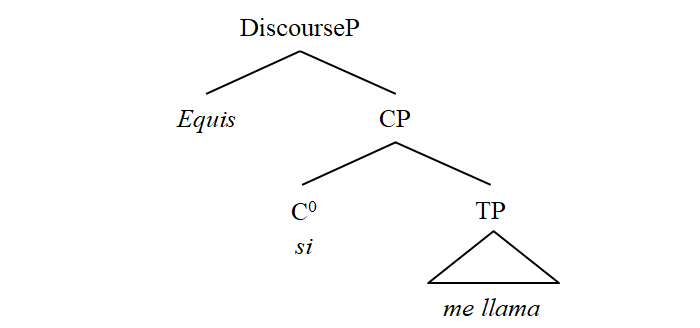
\includegraphics[scale=0.5]{figures/tree3.png}
% \captionof{figure}{\textit{Equis} in si-sentences}
%\end{center}

\begin{figure}
	\caption{\textit{Equis} in si-sentences\label{fig:kellert:tree3}}
	\begin{forest}
		[DiscourseP
			[\textit{Equis}] [CP
				[C\textsuperscript{0}\\\textit{si}][TP
				[\textit{me llama},roof]
		    	]
			]
		]
	\end{forest}
\end{figure}

The focus sensitive operator \textit{if} generates the two alternatives he either will call me or he won’t and \textit{equis} operates on these alternatives in that it expresses indifference whether p or $¬$p is true:

% (56)
\ea\label{ex:kellert:56} Alt(S) = $\lbrace${[}$\lambda$w: he will call me in w{]}; {[}$\lambda$w: $¬$ he will call me in w{]}$\rbrace$
\z

The denotation of \textit{equis} expresses indifference with respect to these alternatives: i.e. he will call me or he won’t call me. There are other uses of \textit{equis} where the QUD is not overtly expressed and the alternatives have to be recovered from the discourse or the common ground as in the following example:

% (57)
\ea\label{ex:kellert:57}
\gll bueno otro dia sigo con el tercer paso. Ay ya \textbf{equis}, que pase lo que tenga que pasar\\
well another day keep with the third step oh now equis that passes that which has to pass\\
\glt ‘Well, I’ll continue next day with the third step. Anyway, come what may’
\z

The analysis suggested for the discourse use of \textit{equis} can be extended to these examples as well as long as it is possible to recover some QUD that triggers alternatives and the speaker signals his indifference with respect to these alternatives. A detailed analysis of such cases awaits future research.
Now that different uses of \textit{equis} in Modern Mexican Spanish have been analyzed, the question arises when these uses emerged in the diachrony.

% 4.
\section{The diachronic change}\label{sec:kellert:4}

% 4.1
\subsection{From variable x into degree predicate \textit{equis}}\label{sec:kellert:4.1}
I assume that the indifference inference of the variable use x has been lexicalized into the meaning of the evaluative predicate \textit{equis} ‘unimportant’.  The variable interpretation is repeated as follows:

% (58)
\ea\label{ex:kellert:58}
\gll Sea un día x (o z).\\
 be-\textsc{subj}-it a day equis (or z)\\
\glt ‘Be it a day x (or z).’\\
Assertion: ◇ $\exists$x $\in$ D {[}day(x) $\wedge$ be (it, x){]} ‘It can be some day’\par
Alternatives = It can be day a $\vee$ It can be day b $\vee$ It can be day c
\z

The pragmatic inference that the hearer derives via conversational maxims is that the speaker is ignorant or indifferent about the identity of the day x. Thus, the variable is not instantiated by some specific day (say Monday):

% (59)
\ea\label{ex:kellert:59} Pragmatic inference in (\ref{ex:kellert:58}): For every x and x is a day, the identity of (x) is not important to the speaker.
\z

I assume that the change from the variable use into the predicate use is triggered by the lexicalization of the pragmatic inference:

% (60)
\ea\label{ex:kellert:60} Lexicalization of the pragmatic inference:\par
	\textit{equis}\textsubscript{<e,t>} = ‘unimportant to the speaker’
\z

In the next step, the lexicalized predicate \textit{equis} turns into degree predicate:

% (61)
\ea\label{ex:kellert:} \textit{equis}\textsubscript{<e,d>} = ‘unimportant to the speaker to degree d’
\z

The next step represents a shift from the speaker’s indifference to indifference of any other attitude holder (e.g. the addressee’s indifference in (\ref{ex:kellert:63}) or 3\textsuperscript{rd} person’s indifference in (\ref{ex:kellert:64})):

% (62)
\ea\label{ex:kellert:64}	equis = ‘unimportant to degree d to some attitude holder’
\ex\label{ex:kellert:63}  Te pareció \textit{equis}? ‘You found it ordinary?’
\ex  Le da \textit{equis}. ‘She does not care.’
\z

The diachronic change of the variable use into degree predicate is thus the result of lexicalization of the pragmatic inference and the shift of speaker’s indifference to indifference of any other attitude holder.


% 4.2
\subsection{From predicate \textit{equis} into discourse adverb \textit{equis}}\label{sec:kellert:4.2}
The diachronic change of \textit{equis} into a discourse adverb is not a very big step. It is just a shift in scope of indifference, i.e. from indifference over identities to indifference over propositions:

% (65)
\ea\label{ex:kellert:65} \textit{Semantic change} of the scope of indifference inference\\
\begin{xlist}
\ex All \textit{entities} are possible options according to speaker’s preferences (diachronic step 1)\\
\ex All \textit{answers} are possible options according to speaker’s preferences (diachronic step 2)
\end{xlist}
\z

This shift in scope of indifference has been lexicalized into a new use of \textit{equis}, namely sentence adverb with a different feature makeup, i.e. \textit{equis} selecting a CP (\sectref{sec:kellert:3.3}). I represent the diachronic change of \textit{equis} schematically as follows. The first diachronic step shows that \textit{equis} has been used as a nominal modifier which has been reanalyzed as a sentence modifier in the second diachronic step (see Figure \ref{fig:kellert:tree4n}):

% (66)
\ea\label{ex:kellert:66} \textit{Syntactic change}\\
\begin{xlist}
\ex	\textit{Equis} used as a nominal modifier (1\textsuperscript{st} diachronic step)\\
\ex	\textit{Equis} used as a sentence modifier (2\textsuperscript{nd} diachronic step)\\
\end{xlist}
\z

% Baum 4
%\begin{center}
%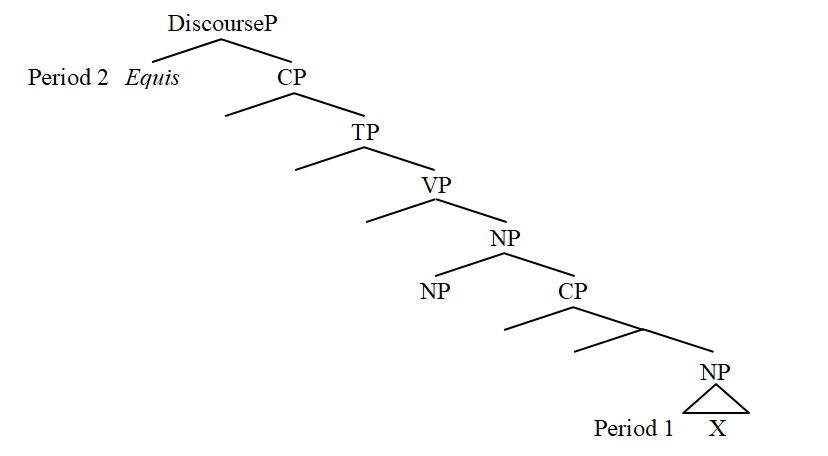
\includegraphics[scale=0.5]{figures/tree4n.png}
% \captionof{figure}{Diachronic shift of discourse adverb \textit{equis}}
%\end{center}
\begin{figure}
	\caption{Diachronic shift of discourse adverb \textit{equis}\label{fig:kellert:tree4n}}
	\begin{forest} nice empty nodes
	[DiscourseP
	[\textit{Equis},name=equis] [CP
	[~] [TP
	[~] [VP
	[~] [NP
	[NP] [CP
	[~] [[~] [NP
	[$X$,roof,name=X]
	]
	]
	]
	]
	]
	]
	]
	]
	\node[left=of equis.base west,anchor=base] {Period 2};
	\node[left=of X.base west,anchor=base] {Period 1};
\end{forest}
\end{figure}

% 4.3
\subsection{Summing up and formulating predictions for corpus analysis}\label{sec:kellert:4.3}
For a diachronic analysis, I have assumed that the variable use of \textit{equis} is the trigger for other uses, namely the discourse adverb use and the predicative/adjectival use. The discourse adverb use is explained as the result of scope shift of speaker’s indifference from nominal to sentential domain. The indifference of the variable x is derived from Gricean conversational maxims. The predictions for the distribution of diachronic data my analysis makes are the following:

\begin{enumerate}
	\item Variable use is expected to precede all other uses.
	\item Variable use is expected to be found in all Spanish varieties and other languages.
	\item Degree predicate use and discourse adverb use are the result of special diachronic processes and thus are not expected to be found in every Spanish variety and every language.
	\item The speaker’s indifference is expected to precede indifference of any other attitude holder (e.g. 3\textsuperscript{rd} person). I thus expect \textit{estuvo equis para mí} ‘it was ordinary/unimportant to me’ to appear before \textit{le parecio equis} ‘she found it unimportant/ordinary.’
	\item I should find the discourse adverb use and the predicative use of \textit{equis} more often in oral and/or informal speech than in formal and written texts as these uses of \textit{equis} lexically encode the speaker’s or the agent’s indifference.
\end{enumerate}

The synchronic data meet predictions 2 and 3 as has been shown in \sectref{sec:kellert:2} (see examples \ref{ex:kellert:7}--\ref{ex:kellert:8}). Other predictions are tested in the following section.

% 5.
\section{Testing the diachronic analysis on diachronic corpus data}\label{sec:kellert:5}
In this section, I will discuss the diachronic distribution of \textit{equis} and investigate the question of when the different synchronic uses of \textit{equis} discussed in \sectref{sec:kellert:2} appeared in diachrony and test the predictions derived from my analysis in \sectref{sec:kellert:4.3}.

The diachronic data was taken from the corpus CDE. I have extracted 163 occurrences of \textit{equis} and classified them according to syntactic and semantic/pragmatic function as for the synchronic \textit{equis} (see \sectref{sec:kellert:2}).

\textit{Equis} increases in relative frequency the in 20\textsuperscript{th} century (see \tabref{tab:3:Equis MexSp. CDE}, rel. freq. value 5.43 in 20\textsuperscript{th} c. against all other values below 1 before the 20\textsuperscript{th} c.). Most occurrences of \textit{equis} in the 20\textsuperscript{th} century can be found in the text genre that represents oral speech (see freq. value of 24.57 in ORAL against other values in other registers below rel. freq. 3 in \tabref{tab:3:Equis MexSp. CDE}).

% Tabelle 3
\begin{table}\footnotesize
\caption{Diachronic distribution of \textit{equis} in CDE subcorpus diachr.}
\label{tab:3:Equis MexSp. CDE}
 \begin{tabularx}{\textwidth}{lCCCCCCCC CCCC}
  \lsptoprule
 & \multicolumn{8}{c}{$n$\textsuperscript{th} c.} & \multicolumn{4}{c}{20\textsuperscript{th} c.}\\\cmidrule(lr){2-9}\cmidrule(lr){10-13}
  Context & 13\textsuperscript{th} &  14\textsuperscript{th} &  15\textsuperscript{th} &  16\textsuperscript{th} &  17\textsuperscript{th} &  18\textsuperscript{th} &  19\textsuperscript{th} & 20\textsuperscript{th} & Acad. & News & Fict. & Oral\\
  \midrule
  Per mil.  & 1.63 & 0.15   & 2.33 & 0.35 & 0.41 & 0.10 & 0.36 & 5.43\cellcolor[gray]{0.8} & 0.60 & 0.60 & 2.94 & 24.57\cellcolor[gray]{0.6}\\
  Total     & 163 & 1 &   19 & 6 & 5 & 1 & 7 & 124\cellcolor[gray]{0.8} & 3 & 3 & 14 & 104\cellcolor[gray]{0.6}\\
  \lspbottomrule
 \end{tabularx}
\end{table}

Before the 20\textsuperscript{th} century, \textit{equis} appears in Latin texts with the meaning ‘horses’ (39 occ. out of 42). Before 20\textsuperscript{th} c., the variable or character use ‘x’ is very infrequent (3 occ. out of 42) in Spanish texts.

% (67)
\ea\label{ex:kellert:67}
\gll en un tiempo <<equis>> anterior perteneció a la persona de Alejandro\\
in a time equis before belonged to the person of Alejandro\\
\glt ‘At some time x in the past, it belonged to the person Alejandro’ (15\textsuperscript{th} c.)
\ex 
\gll En el Semontano hizo muchas equis.\\
in the Semontano made many equis\\
\glt ‘He made many Xs in the Semontano.’ (18\textsuperscript{th} c.)
\ex 
\gll <<por respetos equis o tales>> el hombre no se	opondría a ello, porque era <<de un natural caballero y generoso, y sabía ponerse en todos los casos\\
for respects equis or so the man not it oppose to that because was of a natural gentleman and generous and knew placing in every the cases\\
\glt ‘For some or other reasons, the man won’t be against that because he was a real and generous gentleman and he knew how to react in every case.’ (18\textsuperscript{th} c.)
\z

No discourse adverb use of \textit{equis} was observed until the 20\textsuperscript{th} century.\footnote{As a reviewer has pointed out, the fact that \textit{equis} was not found with a certain function in diachrony does not necessarily mean that this function did not exist at that time, given that the corpus under investigation is relatively small. Therefore, the conclusion about the absence of some function can only be tentative. I agree with this conclusion and suggest drawing a stronger parallel to English \textit{whatever!/whatevs!} in future research, which shows a similar behavior and offers more diachronic data.}
New functions and meanings appear in all varieties in the 20\textsuperscript{th} century: prenominal and postnominal modifier and predicative function of \textit{equis} with the speaker’s ignorance (almost all in the oral register), e.g. \textit{equis razón} ‘some reason but I don’t know which one’ or modifier of quantifier (\textit{cada equis años} ‘every certain year’), \textit{una suma de dinero equis al mes} ‘some amount of money X per month’, \textit{las agencias son equis} ‘the agencies are X’. \textit{Equis} developed a discourse adverb use with the speaker’s indifference in the 20\textsuperscript{th} century (see \sectref{sec:kellert:2}).

The distribution of \textit{equis} is summarized below (see \tabref{tab:4:Summary}) in order to capture different uses of \textit{equis} and their diachronic distribution.

%Tabelle 4
\begin{table}
\caption{Summary of the diachronic data for the analysis\label{tab:4:Summary}}
 \begin{tabularx}{\textwidth}{Qcc}
  \lsptoprule
    Uses of \textit{equis} & before 20\textsuperscript{th} c. & 20\textsuperscript{th} c.\\
  \midrule
   Variable interpretation & $+$ & $+$\\\tablevspace
   Postnominal with evaluative interpretation ‘unremarkable/unimportant’ & $-$ & $+$\\\tablevspace
   Discourse adverb function with  indifference interpretation & $-$ & $+$\\\tablevspace
   Predicative use with degree interpretation (modifiable by degree adverbs ‘very’) & $-$ & $+$\\
  \lspbottomrule
 \end{tabularx}
\end{table}

The diachronic data shows that prediction 1 and prediction 5 are borne out empirically, i.e. the variable use precedes other uses (predicate and discourse use). The text genre prediction is also met, i.e. \textit{equis} appears more often in the oral speech genre. The diachronic data needs to be tested with respect to other predictions in future research, especially prediction 4 about the shift in attitude-holders.

Finally, I would like to address the question whether the shift from variable x into discourse adverb \textit{equis} can be considered as an instance of “subjectification” described in the literature on semantic change (\citealt{Traugott1995}, \citealt{Company2003}, among others). Subjectification is defined as a pragmatic-semantic process whereby “meanings become increasingly based in the speaker’s subjective belief state/attitude toward the proposition”, i.e. towards what the speaker is talking about \citep[31]{Traugott1995}. The diachronic data has shown that the item \textit{equis} was used to mean simply a variable in written texts that do not contain any dialogs or overt linguistic expressions of speaker’s beliefs or attitudes. This restriction changes in 20\textsuperscript{th} century where \textit{equis} starts to be used in oral speech in dialogs that express speaker’s attitudes such as indifference. This change seems to match the subjectification hypothesis. However, I doubt that the speaker’s indifference appeared out of the blue with the use of \textit{equis} in oral speech as the subjectification hypothesis might suggest. The indifference is also present in the variable use of \textit{equis} but in contrast to the discourse use, the indifference is just a pragmatic inference and as such not lexically encoded. I thus assume that the subjectification hypothesis does not fully capture the diachronic process of \textit{equis}.

% 6.
\section{Summary and outlook}\label{sec:kellert:6}
In this article, I have shown different functions of Mexican Spanish \textit{equis} and suggested to analyze them uniformly on the basis of an indifference inference. I started my analysis with \citegen{Fintel2000} notion of indifference derived from the counterfactual inference expressed in English \textit{whatever} free relatives. On my analysis, the variable \textit{equis} or x can also be analyzed in a similar way expressing counterfactual inference, i.e. the speaker is indifferent about which of the values of the variable \textit{equis} or x holds in the actual world. This indifference inference is not lexically encoded in the variable use itself but follows from pragmatic principles. Later in time, the indifference inference shifts towards truth values of propositions and it lexicalizes in the discourse adverb \textit{equis}. The degree predicate \textit{equis} also encodes the indifference inference of the variable \textit{equis} as a lexical property.

I believe that there is a parallel between the diachronic change of \textit{equis} and the shift from \textit{whatever} as an indefinite pronoun (e.g. I grabbed whatever tool was in front of me) to \textit{whatever/whatevs} as discourse adverb in American English which expresses roughly that the speaker does not find it important whether the proposition mentioned previously in the discourse is true or not:

% (70)
\ea\label{ex:kellert:70}
A: \textit{This is true.} B: \textit{Yeah, whatever.}
\z

I will investigate the parallel between the discourse adverb \textit{equis} and \textit{whatever/whatevs} in future research. The diachronic data is taken from the diachronic subcorpus CDE, which does not distinguish between Spanish varieties. In future, it is necessary to look into diachronic corpora that distinguish between varieties.\footnote{I briefly investigated \textit{equis} in the \textit{Corpus Diacrónico y Diatópico del Español de América} (CORDIAM). It contains the total amount of 6,435,906 words from 19 Latin-American countries from 1494 to 1905, with documents from archives, journals and literature. I did not find any use of the discourse adverb or the evaluative predicate as expected. Instead, I found the variable use x referring to some date or number, e.g. \textit{México, x de noviembre, 1578} `Mexico, x/10 of November 1578'.}
In future research, one could also investigate whether \textit{equis} as degree predicate can be modified by other degree modifiers such as modifiers used in comparative clauses. I found some examples on the Internet that need to be checked with native speakers:

%(71)
\ea\label{ex:kellert:71}
\gll sin duda una de las cosas más \textbf{equis} que he visto.\\
without doubt one of the things more equis that have seen\\
\glt ‘No doubt, it’s the most unimportant/unremarkable/worst thing that I’ve ever seen.’ (Internet)
\z

Furthermore, it is necessary to investigate whether degree modification is impossible/ungrammatical with discourse adverb \textit{equis}:

%(72)
\ea\label{ex:kellert:72}
\begin{xlist}
\exi{A:} Some utterance \textit{x}.\\
\exi{B:} \textit{(Muy) equis.}\\
\glt ‘I don’t care about utterance x.’ (to be checked in future)
\end{xlist}
\z

If degree modification is grammatical with discourse adverb \textit{equis}, it should be possible to unify the predicative \textit{equis} and the discourse adverb \textit{equis}. Moreover, I need to account for the meaning ‘several, many’ of \textit{equis} combined with plural nouns (see \sectref{sec:kellert:2.1}).
As \textit{equis} is mostly used in informal speech and many of its uses represent a recent phenomenon, I expect to find speaker variation with the uses of \textit{equis}. Thus, the data need to be checked systematically for speaker variation, too.

%\section*{Abbreviations}
%\section*{Acknowledgements}

{\sloppy\printbibliography[heading=subbibliography,notkeyword=this]}

\end{document}
